\chapter{La Classificazione}
\begin{flushright}\small\textit{Lezione 5 -- 17/03/2026 -- G\'eron, Cap.\ 3}\end{flushright}

\section{Introduzione alla classificazione}
La \textbf{classificazione} è la seconda grande famiglia di metodi del Machine Learning supervisionato. A differenza della regressione, che stima valori continui, la classificazione serve a suddividere i dati in \textbf{categorie discrete}.

\begin{itemize}
    \item \textbf{Classificazione binaria}: due classi mutuamente esclusive (spam/non-spam, gatto/non-gatto, è un 5 / non è un 5).
    \item \textbf{Classificazione multiclasse}: più classi mutuamente esclusive (cifre 0--9, specie di iris).
    \item \textbf{Classificazione multilabel}: più etichette contemporaneamente per la stessa istanza (es.\ riconoscimento facciale in una foto di gruppo: Alice sì, Bob no, Charlie sì).
    \item \textbf{Classificazione multioutput}: ogni etichetta può essere multiclasse (es.\ rimozione del rumore da un'immagine: un'etichetta per pixel, ciascuna da 0 a 255).
\end{itemize}

\section{I dataset storici -- le ``Baseline''}

Le \textbf{baseline} sono dataset standard e famosi usati dai programmatori per testare e confrontare gli algoritmi. Permettono di avere un riferimento condiviso: se un nuovo algoritmo funziona bene su una baseline, ci si può fidare che funzioni anche altrove.

\subsection{Iris Dataset (Fisher, 1936)}

L'\textbf{Iris Dataset} è l'``Hello World'' del Machine Learning. Introdotto nel 1936, è composto da:
\begin{itemize}
    \item \textbf{150 istanze}: 150 fiori di iris analizzati in totale.
    \item \textbf{3 classi (target)}: le tre specie di iris da classificare:
    \begin{itemize}
        \item \emph{Iris Setosa}: caratterizzata da dimensioni relativamente piccole.
        \item \emph{Iris Versicolor}: dimensioni moderate, a metà strada tra le altre due.
        \item \emph{Iris Virginica}: generalmente la più grande tra le tre specie.
    \end{itemize}
    \item \textbf{4 feature}: per ogni fiore sono misurate quattro variabili (in centimetri): lunghezza e larghezza del sepalo, lunghezza e larghezza del petalo.
    \item \textbf{Distribuzione bilanciata}: 50 fiori per specie.
\end{itemize}

È importante nel ML per la sua semplicità (solo 4 attributi), per l'uso come benchmark per confrontare algoritmi diversi, e per studiare l'impatto delle feature su un dataset limitato. In Python è integrato nativamente in \texttt{scikit-learn}.

\subsection{MNIST Dataset (LeCun et al., 1998)}
Il \textbf{MNIST} (Modified National Institute of Standards and Technology) è un dataset molto più complesso, composto da 70\,000 immagini di cifre manoscritte (0--9). Ogni immagine è una griglia di $28 \times 28$ pixel, per un totale di 784 pixel. Le immagini sono in scala di grigi: ogni pixel ha un valore numerico da 0 (bianco) a 255 (nero).

\begin{notebox}[Come ``vede'' la macchina una cifra]
Il software non ha gli occhi per vedere la ``forma'' del numero: analizza una sequenza di 784 numeri (i valori di pixel) e cerca schemi ricorrenti che identifichino la cifra rappresentata. Il dataset è organizzato in una matrice $70\,000 \times 785$ (784 pixel + 1 colonna etichetta).

\textbf{Curiosità storica}: i Babilonesi scrivevano il 3 con tre linee orizzontali e il 2 con due linee. Gli unici numeri che sono rimasti visivamente ``fedeli'' alla loro logica originaria sono lo 0 e l'1.
\end{notebox}

Split ufficiale: \textbf{60\,000 immagini} per il training, \textbf{10\,000} per il test. Il training set è già mescolato casualmente -- questo garantisce che tutti i fold della cross-validation siano simili e che il modello non sia sensibile all'ordine delle istanze.

\begin{notebox}[Scikit-learn e il numero 42]
\textbf{Scikit-learn (sklearn)} è la libreria Python per eccellenza per il ML: contiene algoritmi pronti all'uso e generatori di dataset di prova (permette di generare nuvole di punti artificiali con un certo livello di rumore per testare se un algoritmo riesce a separarle in classi).

Il \textbf{numero 42} compare quasi universalmente come \emph{random seed} nei programmi ML: è una citazione alla saga \emph{Guida Galattica per Autostoppisti}, in cui un super-calcolatore, dopo milioni di anni di calcoli, stabilisce che 42 è ``la risposta alla domanda fondamentale sulla vita, l'universo e tutto quanto''. Fissare il seed garantisce la \textbf{riproducibilità} dei risultati.
\end{notebox}

\section{Rappresentatività e campionamento stratificato}

Uno dei parametri cruciali per la qualità dei dati è la loro \textbf{rappresentatività}. Quando si divide un dataset (per la cross-validation o per il train/test split), le \textbf{proporzioni originali delle classi} devono essere mantenute in ogni sottoinsieme.

Se nel dataset completo i ``5'' sono il 10\% delle immagini, anche in ogni fold di training e test ci deve essere circa il 10\% di ``5''. Questo processo si chiama \textbf{campionamento stratificato} (\emph{stratified sampling}).

\section{Addestrare un classificatore binario}
Riduciamo MNIST a un problema binario: \textbf{``È un 5?''}. Le etichette diventano \texttt{True} (è un 5) o \texttt{False} (non è un 5):

L'algoritmo scelto è lo \textbf{SGDClassifier} (\emph{Stochastic Gradient Descent Classifier}): un classificatore lineare addestrato con la discesa del gradiente stocastica. È molto efficiente su dataset grandi perché processa le istanze una alla volta (aggiornamento incrementale), ed è adatto all'\emph{online learning}.

\section{Metriche di qualità}
\subsection{Perché l'accuratezza da sola non basta}
La valutazione di un classificatore è significativamente più complessa di quella di un regressore. L'\textbf{accuratezza} sembra la metrica naturale:
\[
\text{Accuratezza} = \frac{numero di previsioni corrette}{numero totale di previsioni}= \frac{TP + TN}{TP + TN + FP + FN}
\]
ma può essere ingannevole con dataset \textbf{sbilanciati}.

\begin{itemize}
    \item se il classificatore è perfetto (solo TP e TN) allora l'accuratezza è 1 (100\%)
    \item se il classificatore sbaglia tutto (solo FP e FN) allora l'accuratezza è 0
\end{itemize}

\begin{warnbox}[Il paradosso del classificatore stupido]
Nel dataset MNIST, solo circa il 10\% delle immagini sono ``5''. Un classificatore banale che risponde \emph{sempre} ``non è un 5'' ottiene il \textbf{90\% di accuratezza} -- senza aver imparato nulla di utile. L'accuratezza da sola non è sufficiente per valutare un classificatore su classi sbilanciate. Servono metriche più informative: \textbf{precisione}, \textbf{recall}, \textbf{F1}.
\end{warnbox}

\subsection{Matrice di confusione}

La \textbf{matrice di confusione} è lo strumento fondamentale per valutare un classificatore: conta quante volte le istanze di ogni classe reale vengono predette come ogni possibile classe.

\begin{center}
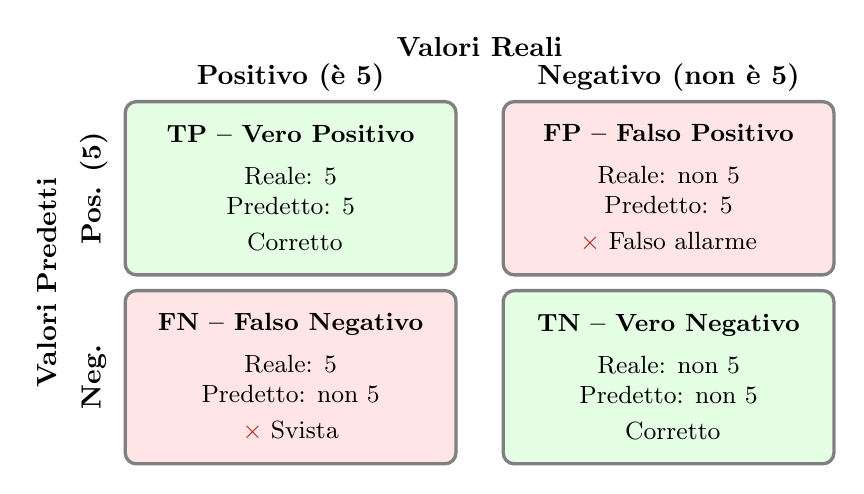
\begin{tikzpicture}[font=\small]
    \node[rectangle, draw=gray, fill=green!10, very thick, rounded corners,
          minimum width=4.2cm, minimum height=2.2cm, align=center] (TP)
          at (-2.4, 1.0) {\textbf{TP -- Vero Positivo}\\[4pt]\small Reale: 5\\Predetto: 5\\[2pt]\textcolor{OliveGreen}{\checkmark} Corretto};

    \node[rectangle, draw=gray, fill=red!10, very thick, rounded corners,
          minimum width=4.2cm, minimum height=2.2cm, align=center] (FP)
          at (2.4, 1.0) {\textbf{FP -- Falso Positivo}\\[4pt]\small Reale: non 5\\Predetto: 5\\[2pt]\textcolor{BrickRed}{$\times$} Falso allarme};

    \node[rectangle, draw=gray, fill=red!10, very thick, rounded corners,
          minimum width=4.2cm, minimum height=2.2cm, align=center] (FN)
          at (-2.4, -1.4) {\textbf{FN -- Falso Negativo}\\[4pt]\small Reale: 5\\Predetto: non 5\\[2pt]\textcolor{BrickRed}{$\times$} Svista};

    \node[rectangle, draw=gray, fill=green!10, very thick, rounded corners,
          minimum width=4.2cm, minimum height=2.2cm, align=center] (TN)
          at (2.4, -1.4) {\textbf{TN -- Vero Negativo}\\[4pt]\small Reale: non 5\\Predetto: non 5\\[2pt]\textcolor{OliveGreen}{\checkmark} Corretto};

    \node[font=\bfseries] at (0, 2.8) {Valori Reali};
    \node[font=\bfseries] at (-2.4, 2.4) {Positivo (è 5)};
    \node[font=\bfseries] at (2.4, 2.4) {Negativo (non è 5)};
    \node[rotate=90, font=\bfseries] at (-5.5, -0.2) {Valori Predetti};
    \node[rotate=90, font=\bfseries] at (-4.9, 1.0) {Pos. (5)};
    \node[rotate=90, font=\bfseries] at (-4.9, -1.4) {Neg.};
\end{tikzpicture}
\end{center}

\begin{itemize}
    \item Un \textbf{TP mancato} diventa un FN (svista).
    \item Un \textbf{TN mancato} diventa un FP (falso allarme).
\end{itemize}

\subsection{Precisione}

La \textbf{precisione} risponde alla domanda: ``dei campioni che il modello ha classificato come positivi, quanti erano davvero positivi?''. Penalizza i \textbf{falsi allarmi} (FP).

\begin{equation}
P = \frac{TP}{TP + FP}
\end{equation}

Alta precisione $\Rightarrow$ pochi falsi positivi. Utile quando un falso allarme è costoso.

\begin{exbox}[Filtro spam: alta precisione]
Un'email importante classificata come spam è un disastro. Preferiamo lasciare passare qualche spam (basso recall) piuttosto che bloccare email legittime. Il costo del FP (email legittima persa) è molto alto.
\end{exbox}


\subsection{Recall (Sensibilità)}
Il \textbf{recall} (o \emph{sensibilità} / \emph{True Positive Rate}) risponde alla domanda: ``dei campioni che erano davvero positivi, quanti ne abbiamo recuperati?''. Penalizza le \textbf{sviste} (FN).

\begin{equation}
R = \frac{TP}{TP + FN}
\end{equation}

Alto recall $\Rightarrow$ pochi falsi negativi. Utile quando perdere un positivo è costoso.

\begin{exbox}[Screening tumorale: alto recall]
Nessun paziente malato deve essere classificato come sano (FN = tumore non rilevato). Accettiamo molti falsi positivi (pazienti sani rimandati per ulteriori esami): il costo del FP è basso, il costo del FN è altissimo.
\end{exbox}

\subsection{Il trade-off Precisione -- Recall}
Precisione e recall sono in \textbf{tensione}: aumentare l'una tende a ridurre l'altra. Questo dipende dalla \textbf{soglia di decisione} (\emph{threshold}) del classificatore.

\begin{center}
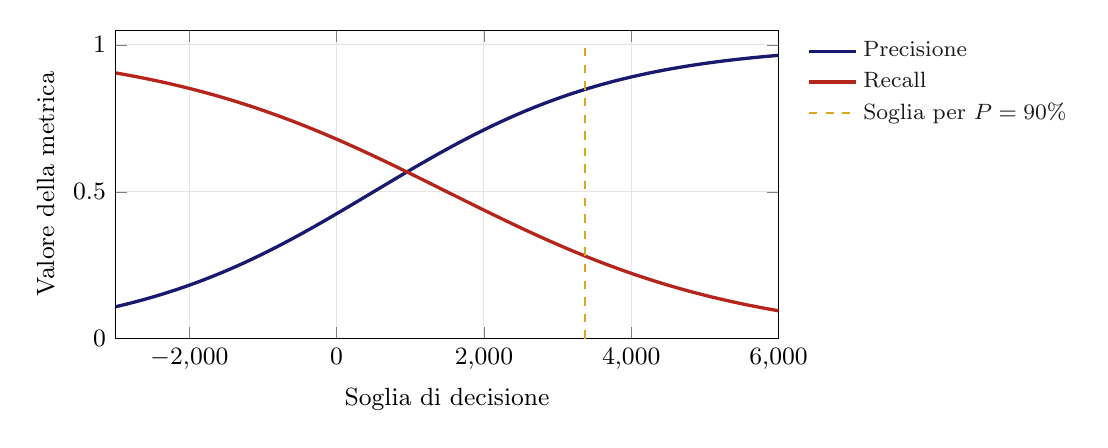
\begin{tikzpicture}[font=\small]
\begin{axis}[
    width=10cm, height=5.5cm,
    xlabel={Soglia di decisione},
    ylabel={Valore della metrica},
    xmin=-3000, xmax=6000, ymin=0, ymax=1.05,
    grid=major, grid style={gray!20},
    legend pos=outer north east,
    legend style={font=\footnotesize, cells={anchor=west}, 
                  legend columns=1, draw=none, fill=white, fill opacity=0.9},
    legend cell align={left}
]
\addplot[very thick, MidnightBlue, domain=-3000:6000, samples=200]
    {1/(1+exp(-0.0006*(x-500)))};
\addlegendentry{Precisione}
\addplot[very thick, BrickRed, domain=-3000:6000, samples=200]
    {1 - 1/(1+exp(-0.0005*(x-1500)))};
\addlegendentry{Recall}
\addplot[thick, Goldenrod, dashed] coordinates {(3370,0)(3370,1.0)};
\addlegendentry{Soglia per $P = 90\%$}
\end{axis}
\end{tikzpicture}
\end{center}

\begin{itemize}
    \item \textbf{Alzare la soglia} $\to$ il classificatore è più ``selettivo'' nel dichiarare positivo: \textbf{precisione aumenta}, \textbf{recall diminuisce}.
    \item \textbf{Abbassare la soglia} $\to$ il classificatore è più ``permissivo'': \textbf{recall aumenta}, \textbf{precisione diminuisce}.
\end{itemize}


\subsection{F1-Score}
Quando si vuole una \textbf{singola metrica} che bilanci precisione e recall (utile per confrontare due classificatori), si usa l'\textbf{F1-Score}: la \emph{media armonica} tra $P$ e $R$.

\begin{equation}
F_1 = 2 \cdot \frac{P \cdot R}{P + R} = \frac{2\,TP}{2\,TP + FP + FN}
\end{equation}

La \textbf{media armonica} penalizza fortemente i valori bassi: $F_1$ è alto \emph{solo se entrambi} $P$ e $R$ sono alti. Se uno dei due è basso, l'F1 crolla.

\begin{center}
\renewcommand{\arraystretch}{1.3}
\begin{tabular}{@{} l c c c @{}}
\toprule
\textbf{Scenario} & \textbf{Precisione} & \textbf{Recall} & \textbf{F1} \\
\midrule
Entrambi alti & 90\% & 85\% & 87{,}4\% \\
Uno alto, uno basso & 95\% & 20\% & 33{,}1\% \\
Entrambi medi & 70\% & 70\% & 70{,}0\% \\
\bottomrule
\end{tabular}
\end{center}

\begin{exbox}[F1 sull'SGD 5-detector reale]
$F_1 = 2 \times (0{,}837 \times 0{,}651) / (0{,}837 + 0{,}651) \approx 0{,}733$

Il classificatore ha una precisione accettabile ma un recall basso -- solo il 65\% dei ``5'' viene rilevato. L'F1 di 73\% riflette questo squilibrio.
\end{exbox}

\begin{thmbox}[In sintesi: quale metrica scegliere?]
Nessuna singola metrica racconta tutta la storia. Il principio guida è \emph{pensare al costo} di FN vs.\ FP nel dominio applicativo:
\begin{itemize}
    \item \textbf{Sanità / sicurezza}: privilegiare il \textbf{recall} (nessun caso positivo deve sfuggire).
    \item \textbf{Spam / content filtering}: privilegiare la \textbf{precisione} (nessun falso allarme).
    \item \textbf{Confronto generale tra classificatori}: usare l'\textbf{F1} come metrica di compromesso.
    \item \textbf{Dataset sbilanciati}: evitare l'accuratezza da sola; preferire F1, PR-curve, o ROC-AUC.
\end{itemize}
\end{thmbox}